\documentclass[tikz,border=3pt]{standalone}
\usepackage[utf8]{inputenc}
\usepackage[T1]{fontenc}
\usepackage{lmodern}
\renewcommand{\familydefault}{\sfdefault}
\usepackage{sansmath}\sansmath
\usepackage{chemfig}
\usepackage{pgfplots}\pgfplotsset{compat=1.18,/pgf/number format/use comma,/pgf/number format/1000 sep={.}}
\usetikzlibrary{arrows.meta,calc,positioning,decorations.pathmorphing,patterns}
% paleta del sitio
\definecolor{nar}{HTML}{E8680C}\definecolor{narc}{HTML}{FFB35C}\definecolor{hielo}{HTML}{FFF3E8}
\definecolor{tinta}{HTML}{1D1D1F}\definecolor{gris}{HTML}{6E6E73}\definecolor{lila}{HTML}{7C5CF0}
\definecolor{azul}{HTML}{2F6FD6}\definecolor{menta}{HTML}{17A673}\definecolor{coral}{HTML}{E8342A}
\begin{document}
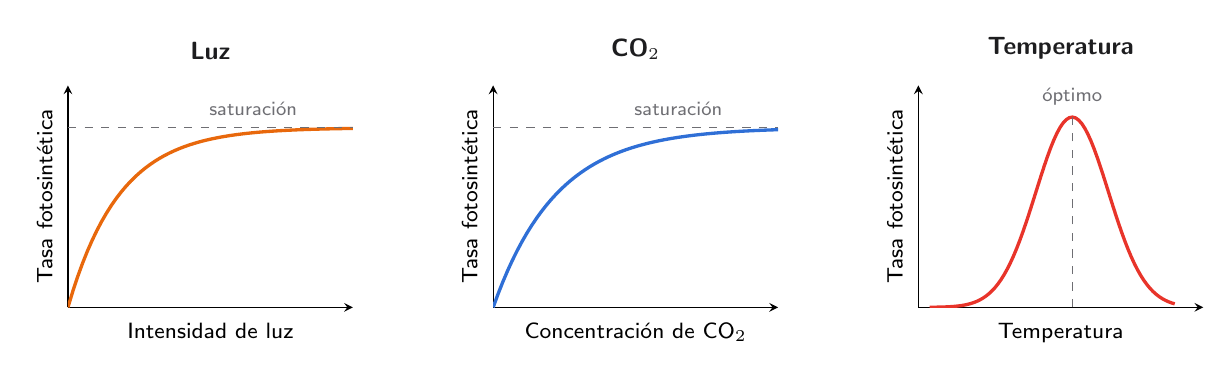
\begin{tikzpicture}[font=\small]
\pgfplotsset{mini/.style={width=5.2cm,height=4.4cm,axis lines=left,xtick=\empty,ytick=\empty,ymin=0,ymax=10.5,xmin=0,xmax=10,ylabel={Tasa fotosintética},ylabel style={font=\footnotesize},xlabel style={font=\footnotesize},title style={font=\small\bfseries,text=tinta}}}
\begin{axis}[mini,at={(0,0)},title={Luz},xlabel={Intensidad de luz}]
\addplot[nar,very thick,domain=0:10,samples=60] {8.5*(1-exp(-0.55*x))};
\addplot[gris,dashed] coordinates {(0,8.5)(10,8.5)};
\node[font=\scriptsize,text=gris,anchor=south] at (axis cs:6.5,8.6) {saturación};
\end{axis}
\begin{axis}[mini,at={(5.4cm,0)},title={CO$_2$},xlabel={Concentración de CO$_2$}]
\addplot[azul,very thick,domain=0:10,samples=60] {8.5*(1-exp(-0.45*x))};
\addplot[gris,dashed] coordinates {(0,8.5)(10,8.5)};
\node[font=\scriptsize,text=gris,anchor=south] at (axis cs:6.5,8.6) {saturación};
\end{axis}
\begin{axis}[mini,at={(10.8cm,0)},title={Temperatura},xlabel={Temperatura},xmax=50]
\addplot[coral,very thick,domain=2:45,samples=80] {9*exp(-((x-27)/9)^2)};
\addplot[gris,dashed] coordinates {(27,0)(27,9)};
\node[font=\scriptsize,text=gris,anchor=south] at (axis cs:27,9.1) {óptimo};
\end{axis}
\end{tikzpicture}
\end{document}
